%!TeX root = ./../Thesis.tex

%##########################################################
% Inhalt
%##########################################################
\chapter{Grundlagen}\label{chap:basics}
Dieses Kapitel ist zur Vermittlung von technischen Grundlagen, um im Verlauf der Arbeit angewandte Technologien zu verstehen und umgesetzte Lösungsversuche nachvollziehen zu können. Dabei wird Fokus auf das Thema der LLM's, dem \textit{Prompt Engineering} sowie \textit{SonarQube} gelegt. Der SDLC wird noch einmal genauer erläutert, um die Einordnung des Testens im Entwicklungsalltag zu verdeutlichen. Da \textit{Unit-Tests} einen wichtigen Bestandteil der Arbeit repräsentieren, werden Grundlagen zu diesen Tests geschaffen und der Bezug zur Programmiersprache \textit{Java} hergestellt.

\section{Software Development Lifecycle}
Der SDLC ist ein Grundlagenzyklus, welcher innerhalb eines Softwareprojektes festgelegt und während der Bearbeitung des Projektes befolgt wird. \cite*{SoftwareDevelopmentLife} Dieser dient zur Verbesserung von Qualität und Entwicklung.\begin{figure}[ht]
    \centering
    \tikzstyle{block} = [circle, draw, text width=3.2em, text centered, rounded corners, minimum height=3em, font=\small]
    \begin{tikzpicture}
        \tikzset{node distance = 0.75cm and 2.0cm}
        \node (n1) at (0,0) [block]  {Plan};
        \node (n2) [block, below right=0.5cm and 1.5cm of n1] {Design};
        \node (n3) [block, below left=1.5cm and 0cm of n2] {Develop};
        \node (n5) [block, below left=0.5cm and 1.5cm of n1] {Deploy};
        \node (n4) [block, below right=1.5cm and 0cm of n5] {Test};
        % Connectors
        \draw [->, thick] (n1) -- (n2);
        \draw [->, thick] (n2) -- (n3);
        \draw [->, thick] (n3) -- (n4);
        \draw [->, thick] (n4) -- (n5);
        \draw [->, thick] (n5) -- (n1);
    \end{tikzpicture}
    \caption{Phasen eines SDLC}
    \label{fig:sdlc}
\end{figure}Ein typischer SDLC besteht aus 6 verschiedenen Phasen. [Abb. \ref{fig:sdlc}]\\\\
\textbf{Planung}\\[0.2cm]
Eine Planung erfolgt in der Regel durch eine neue Innovation, welche von einem Endnutzer oder Sponsor ausgeht. \cite*{tikySoftwareDevelopmentLife} Hierbei werden Projektumfang, Ziele sowie Anforderungen definiert. Dabei steht vor allem der Projektplan im Fokus, welcher Zeitrahmen und Ressourcen definiert. \cite*{hossainSoftwareDevelopmentLife2023}\\\\
\textbf{Entwurf}\\[0.2cm]
In der Entwurfsphase wird festgelegt, wie benötigte Softwarekomponenten zusammenwirken und eine Produktarchitektur definiert. Es kommt zum Entwerfen des \textit{User Interfaces} (engl. Benutzeroberfläche) mit Blick auf die \textit{User Experience} (engl. Benutzererfahrung). \cite*{hossainSoftwareDevelopmentLife2023}\\\\
\textbf{Entwicklung und Implementierung}\\[0.2cm]
Nach Abschluss aller vorher nötigen Phasen, beginnen Programmierer mit der Entwicklung und Implementation der Software bei Einhaltung aller festgelegten Anforderungen und entsprechend dem Architekturentwurf. \cite*{tikySoftwareDevelopmentLife} \\\\
\textbf{Testen}\\[0.2cm]
Das Testen der Software ist eine wichtige und essenzielle Phase, die während sowie nach der Entwicklung stattfindet. Hierbei kommt es zur Durchführung verschiedener Teststufen, einschließlich \textit{Unit-Tests}, \textit{Integration-Tests}, \textit{System-Tests} und Benutzerakzeptanz-Tests. Es werden Fehler identifiziert und behoben sowie Anforderungen aus vorherigen Phasen überprüft. \cite*{hossainSoftwareDevelopmentLife2023}\\\\
\textbf{Deployment und Wartung}\\[0.2cm]
Zum \textit{Deployment} gehört die Bereitstellung der Software in einer \textit{Staging}-Umgebung. Diese wird vorausgesetzt, um abschließende Tests durchzuführen und die Software zu validieren. Es werden Server und Datenbanken konfiguriert, sodass eine Produktionsumgebung vorbereitet wird. Nach erfolgreichen \textit{Rollout} (engl. ausrollen) der Software steht die Überwachung und Wartung der Produktionsumgebung im Fokus. \cite*{hossainSoftwareDevelopmentLife2023}\\\\
Insbesondere die Phase des Testens sollte als eine \textit{Sub stage} (engl. Unterstufe) aller Phasen betrachtet werden, da ein Testen von Anforderungen, Implementation, Code sowie \textit{Deployment} dauerhaft notwendig ist. Aufgrund dessen ist die Testphase besonders komplex und aufwändig, weshalb der Fokus ständig aufrechterhalten werden muss. \cite*{tikySoftwareDevelopmentLife}

\section{Large Language Models}
\subsection{Begriff und Einführung}
Hinter dem simplen Begriff \textit{Large Language Model} steckt eine komplizierte Technologie mit großer Herkunftsgeschichte, welche eine Definition mehrerer Begrifflichkeiten im Feld der Künstlichen Intelligenz (kurz KI) voraussetzt. Dadurch kann ein Grundverständnis geschaffen werden, um den Begriff LLM besser einordnen zu können. \cite{seemannKuenstlicheIntelligenzLarge} \\\\ Ein Hauptbestandteil der KI spielen Künstliche Neuronale Netze (kurz \acs{KNN}). 
Die Inspiration dieser Netze entstammt dem Neuronalen Netzwerk im Gehirn eines Menschen. \cite*{seemannKuenstlicheIntelligenzLarge} Das Ziel dabei ist, natürliche Organismen nachzubauen, und somit lernfähige Programme zu erzeugen. 
\begin{figure}[ht]
    \centering
    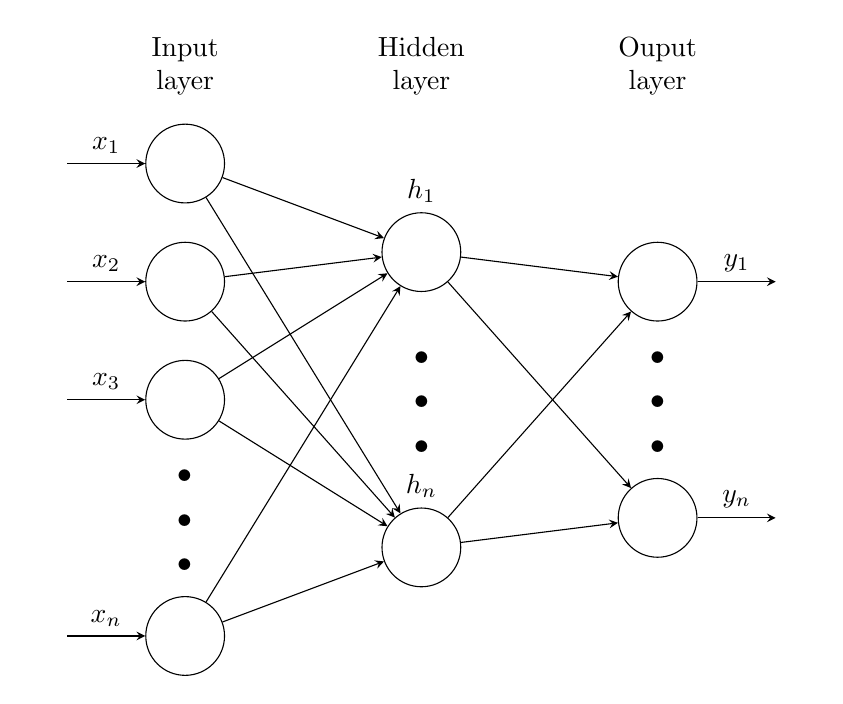
\begin{tikzpicture}[x=1.5cm, y=1.5cm, >=stealth]
        \tikzset{%
         every neuron/.style={
            circle,
            draw,
            minimum size=1cm},
        neuron missing/.style={
            draw=none, 
            scale=4,
            text height=0.333cm,
            execute at begin node=\color{black}$\vdots$},
        }
        
        \foreach \m/\l [count=\y] in {1,2,3,missing,4}
        {
            \node [every neuron/.try,neuron \m/.try] (input-\m) at (0,2.5-\y) {};
        }       
        \foreach \m [count=\y] in {1,missing,2}
            \node [every neuron/.try, neuron \m/.try ] (hidden-\m) at (2,2-\y*1.25) {};

        \foreach \m [count=\y] in {1,missing,2}
            \node [every neuron/.try, neuron \m/.try ] (output-\m) at (4,1.5-\y) {};

        \foreach \l [count=\i] in {1,2,3,n}
            \draw [<-] (input-\i) -- ++(-1,0)
                node [above, midway] {$x_\l$};

        \foreach \l [count=\i] in {1,n}
            \node [above] at (hidden-\i.north) {$h_\l$};

        \foreach \l [count=\i] in {1,n}
            \draw [->] (output-\i) -- ++(1,0)
                node [above, midway] {$y_\l$};

        \foreach \i in {1,...,4}
        \foreach \j in {1,...,2}
            \draw [->] (input-\i) -- (hidden-\j);

        \foreach \i in {1,...,2}
        \foreach \j in {1,...,2}
            \draw [->] (hidden-\i) -- (output-\j);

        \foreach \l [count=\x from 0] in {Input, Hidden, Ouput}
            \node [align=center, above] at (\x*2,2) {\l \\ layer};
    \end{tikzpicture}
    \caption{Grundlegender Aufbau eines KNN}
    \label{fig:knn}
\end{figure}Der Aufbau eines solchen Netzes folgt dem Vorbild der Struktur des menschlichen Gehirns und besteht somit aus verbundenen künstlichen Nervenzellen (Neuronen), welche durch eine Eingabeschicht passende Ausgaben erzeugen. \cite*{morrKuenstlicheNeuronaleNetze} Unterschieden wird zwischen 3 verschiedenen Arten von Neuronen. Somit besteht ein Netz grundlegend aus \textit{Input-}, \textit{Hidden-} und \textit{Output}-Neuronen, zwischen denen eine gewichtete Verbindung herrschen kann. \cite*{NeuronaleNetzeEinfuhrung} [Abb. \ref{fig:knn}] Durch solch eine Struktur können KNN durch maschinelles Lernen mit großen Datenmengen trainiert werden und dadurch Fähigkeiten wie das Generieren von Texten erlernen. \cite*{seemannKuenstlicheIntelligenzLarge}\\\\ Ein weiteres Teilgebiet in der KI ist das \textit{Natural Language Processing} (engl. natürliche Sprachverarbeitung, kurz NLP). Hierbei liegt der Fokus auf der Interaktion zwischen Computern und menschlicher Sprache, in dem Algorithmen und Modelle ermöglichen, dass Computer die menschliche Sprache verstehen, interpretieren und auf sinnvolle Weise erzeugen können. \cite*{muruganNaturalLanguageProcessing2024} \\\\ Dies schafft die Grundlage eines \textit{Large Language Models}, denn diese Modelle basieren auf KNN und sind spezialisiert auf die natürliche Sprachverarbeitung. \cite*{seemannKuenstlicheIntelligenzLarge} Sie sind ausgelegt, um Beziehungen zwischen einzelnen Daten zu lernen und Sequenzen vorherzusagen. Insbesondere deswegen sind sie für die Generierung von Text in natürlicher Sprache geeignet, da sie die Fähigkeit besitzen Sprache aus großen Datensätzen von geschriebenen Texten im Internet sowie digitalisierten Büchern zu erlernen, um sich in neuartigen Situationen angepasst verhalten zu können. \cite*{okerlundWhatChatterbox2022} \cite*{authorityofthehouseoflordsLargeLanguageModels} \\Ein \textit{pre training} (engl. Vortraining) sowie \textit{fine tuning} (engl. Feinabstimmung) ist in vielen Fällen notwendig, um die Genauigkeit des Modells auf bestimmte Bereiche zu verbessern. \cite{HowLLMsWork} Um eine solche Genauigkeit zu gewährleisten, arbeiten Sprachmodelle mit dem Prinzip der \textit{Tokenisierung}. Im Rahmen dieses Vorverarbeitungsschritts erfolgt eine Zerlegung des Textes in Token, wobei diese aus Zeichen, Teilwörtern oder Symbolen bestehen können. \cite*{naveedComprehensiveOverviewLarge2024} \\ Grundlegend nehmen LLM's einen \textit{Prompt} als Eingabe entgegen und generieren abhängig von gesetzten Parametern des Modells, sowie bisher erlernten Informationen, eine Ausgabe. \begin{figure}[ht]
    \centering
    \tikzstyle{block} = [rectangle, draw, text width=5em, text centered, rounded corners, minimum height=3em, font=\small]
    \begin{tikzpicture}
        \tikzset{node distance = 0.75cm and 2.0cm}
        \node (n1) at (0,0) [rectangle, text width=5em, text centered, rounded corners, minimum height=3em]  {\colorbox{gray!25}{Es}};
        \node (n2) [block, above=of n1] {Wahrscheinlichkeitsverteilung};
        \node (n3) [block, above=of n2] {Sampling Strategy};
        \node (n4) [rectangle, text width=5em, text centered, rounded corners, minimum height=3em, above=of n3] {\colorbox{gray!25}{ist}};
        \node (n5) [rectangle, text width=5em, text centered, rounded corners, minimum height=3em, right=of n1] {\colorbox{gray!25}{Es ist}};
        \node (n6) [block, right=of n2] {Wahrscheinlichkeitsverteilung};
        \node (n7) [block, right=of n3] {Sampling Strategy};
        \node (n8) [rectangle, text width=5em, text centered, rounded corners, minimum height=3em, right=of n4] {\colorbox{gray!25}{ein}};
        \node (n9) [text width=5em, text centered, right=of n5] {\colorbox{gray!25}{Es ist ein}};
        \node (n10) [block, right=of n6] {Wahrscheinlichkeitsverteilung};
        \node (n11) [block, right=of n7] {Sampling Strategy};
        \node (n12) [rectangle, text width=5em, text centered, rounded corners, minimum height=3em, right=of n8] {\colorbox{gray!25}{schöner}};
        % Connectors
        \draw [->, thick] (n1) -- (n2);
        \draw [->, thick] (n2) -- (n3);
        \draw [->, thick] (n3) -- (n4);
        \draw [->, thick] ($(n4.east) - (0.35,0)$) -| ($(n4.east) + (1.0,0)$) |- ($(n5.west) - (1.0,0)$) -- (n5);
        \draw [->, thick] (n5) -- (n6);
        \draw [->, thick] (n6) -- (n7);
        \draw [->, thick] (n7) -- (n8);
        \draw [->, thick] ($(n8.east) - (0.35,0.0)$) -| ($(n8.east) + (1.0,0)$) |- ($(n9.west) - (1.0,0)$) -- (n9);
        \draw [->, thick] (n9) -- (n10);
        \draw [->, thick] (n10) -- (n11);
        \draw [->, thick] (n11) -- (n12);
        \draw [->, thick] ($(n12.east) + (-0.25,0)$) -- ($(n12.east) + (0.5,0)$);
        \draw [->, thick] ($(n1.east) - (0.35,0)$) -- (n5);
        \draw [->, thick] (n5) -- (n9);
    \end{tikzpicture}
    \caption{Wordgenerierung in LLMs}
    \label{fig:word}
\end{figure}Das vorhergesagte Wort ist das Ergebnis einer Wahrscheinlichkeitsverteilung des Modells und wird so lange mit der Sequenz verknüpft, bis sie endgültig ist. [Abb. \ref{fig:word}] Dabei können unterschiedliche Ergebnisse erzielt werden, welche abhängig von der \textit{sampling strategy} (engl. Stichprobenstrategie) sind. \cite*{cholletDeepLearningPython2018} Ein Beispiel wäre \textit{sampling with temperature} (engl. Stichprobeverfahren mit Temperatur-Parameter), bei dem die Wahl der Temperatur entscheidungsgebend ist. Wählt man bspw. einen Wert nahe 0, so wird das Sprachmodell in den meisten Fällen das Ergebnis mit der höchsten Wahrscheinlichkeit nutzen. Umso höher der Wert, desto eher wird das Ergebnis mit einer niedrigeren Wahrscheinlichkeit genutzt. \cite*{WeightsBiases} Dies bedeutet, um auf die Qualität der Ergebnisse Einfluss zu nehmen, gibt es die Möglichkeit manuelle Parameter zu setzen. Darunter zählen z.B. \textit{max tokens} zum Festlegen der maximalen Anzahl an Tokens die generiert werden dürfen oder auch, wie oben erwähnt, die Temperatur, welche die Zufälligkeit von 0.0 (deterministisch) - 2.0 (extrem zufällig) regelt.\\ Im Allgemeinen finden LLM's eine große Spannbreite an Anwendung, wie bspw. Textgenerierung, Vervollständigung und Zusammenfassung. \cite*{dhadukHowLargeLanguage2023}

\subsection{Generative Pre-trained Transformer}\label{subsection:gpt}
Unter allen Sprachmodellen, wie bspw. FLAN oder PaLM, sticht die Serie der \textit{Generative Pre-trained Transformer} (engl. vortrainierter generativer Transformator, kurz GPT) durch ihre besonders hohe Performance hervor. \cite*{yeComprehensiveCapabilityAnalysis2023} Die in GPT verwendete Transformer-Architektur ist ein bedeutender Fortschritt gegenüber früheren \acs{NLP}-Ansätzen. Durch ihren Mechanismus der Selbstbeobachtung ermöglicht sie es dem Modell, bei der Wortgenerierung, den Kontext des gesamten Satzes zu berücksichtigen. \cite*{yenduriGenerativePretrainedTransformer2023} \\ \textit{OpenAI's} Sprachmodelle sind Teil dieser Serie und haben mit \textit{GPT-3.5 Turbo}, \textit{GPT-4} sowie \textit{GPT-4o} drei der populärsten LLM's auf den Markt gebracht. \cite*{yaoSurveyLargeLanguage2024}\\
\textit{GPT-4o} ist das am weitesten fortgeschrittene Modell. Neben seiner Multimodalität besitzt es die gleiche Intelligenz wie \textit{GPT-4}, ist jedoch viel effizienter. Es erzeugt Text doppelt so schnell, ist 50\% billiger und ebenso das aktuellste Modell von OpenAI. Somit rückt \textit{GPT-4o} in den Fokus dieser Arbeit. \cite*{OpenAIPlatform} Tabelle \ref{fig:gpt} zeigt alle relevanten Daten und Fakten des LLM.
\bgroup
\def\arraystretch{2}
\begin{table}[!h]
	\vspace{.5cm}
	\begin{center}
		\begin{tabular}{|c||c|c|}
			\hline 
			& GPT-4o \\
			\hline 
			\hline
			Kontext-Fenster & 128.000 Token \\
			\hline
			Maximaler Output & 4.096 Token 
			 \\
			\hline
			Input Kosten & \$5.00 / 1M Token \\
			\hline
			Output Kosten & \$15.00 / 1M Token \\
			\hline
		\end{tabular} 
	\end{center}
	\caption{Grundlegender Vergleich beider GPT-Modelle}
	\label{fig:gpt}
\end{table}
\egroup


\section{Prompt Engineering}
Das \textit{Prompt-Engineering} spiegelt eine Technik zur Verbesserung der Fähigkeiten von LLM's wieder. Es werden sogenannte \textit{Prompts} genutzt, welche eine strategische und spezifische Anweisung repräsentieren, um die Modellausgabe zu steuern. Somit wird ein Mechanismus bereitgestellt, der ein \textit{fine tuning} der Ausgabe ermöglicht und das Modell anpassungsfähiger macht. \cite*{sahooSystematicSurveyPrompt2024} \begin{figure}[ht]
    \vspace{.5cm}
    \centering
    \tikzstyle{block} = [rectangle, draw, text width=7.5em, text centered, align=center, inner sep=1ex, rounded corners, font=\small]
    \begin{tikzpicture}
        \tikzset{node distance = 0.75cm and 1.5cm}
        % Main node with embedded tikzpicture
        \node (n1) at (0,0) [block, minimum height=4em, text depth=0.5em, inner sep=1ex] {
            \begin{tikzpicture}[node distance=0.25cm]
                \node (n1a) [minimum height=1.5em, inner sep=1ex] {\textbf{\textit{Prompt}}};
                \node (n1b) [block, text width=6em, minimum height=1.5em, inner sep=1ex, below=of n1a] {Anweisung};
                \node (n1c) [block, below=of n1b, text width=6em, minimum height=1.5em, inner sep=1ex] {Kontext};
                \node (n1d) [block, below=of n1c, text width=6em, minimum height=1.5em, inner sep=1ex] {Eingabedaten};
                \node (n1e) [block, below=of n1d, text width=6em, minimum height=1.5em, inner sep=1ex] {Ausgabeindikator};
            \end{tikzpicture}
        };
        \node (n2) [block, minimum height=4em, text depth=0em, inner sep=2ex, right=of n1] {
            \begin{tikzpicture}[node distance=1.25cm]
                \node (n2a) [block, text width=4em, minimum height=1.5em, inner sep=1ex] {\textbf{LLM}};
                \node (n2b) [block, text width=4em, minimum height=1.5em, inner sep=1ex, below=of n2a] {\textit{training on parameters}};
                \draw [->, thick, dashed] ($(n2a.south) - (0.8,0.0)$) -- ($(n2b.north) - (0.8,0.0)$);
                \draw [->, thick, dashed] ($(n2b.north) + (0.8,0.0)$) -- ($(n2a.south) + (0.8,0.0)$);
            \end{tikzpicture}
        };
        \node (n3) [block, right=of n2] {Ausgabe};
        % Connectors
        \draw [->, thick] (n1) -- (n2);
        \draw [->, thick] (n2) -- (n3);
    \end{tikzpicture}
    \caption{\textit{Prompt Engineering} Prozess }
    \label{fig:prompt-eng}
\end{figure}


\subsection{Prompt Elemente}
Der Aufbau eines \textit{Prompts} besteht aus folgenden Elementen [Abb. \ref{fig:prompt-eng}]:
\begin{itemize}
    \setlength{\parskip}{1pt}
    \item \textbf{Anweisung} - eine Anweisung, die das Modell ausführen soll
    \item \textbf{Kontext} - Zusatzkontext, der das Modell zu besseren Antworten lenken kann
    \item \textbf{Eingabedaten} - die Eingabe, für die eine Antwort gefunden werden soll
    \item \textbf{Ausgabeindikator} - das Format der Ausgabe
\end{itemize}
Es sind nicht alle Elemente nötig um einen \textit{Prompt} zu kreieren, bspw. benötigt es keinen Kontext, wenn die Eingabedaten für genug Klarheit schaffen. \cite*{ElementsPromptNextra2024}

\subsection{Prompt Techniken}
Wenn Aufgaben an Größe und Komplexität zunehmen, erzielt ein einfacher \textit{Prompt} in den meisten Fällen nicht das gewünschte Ergebnis. Zur Behebung dieses Problems gibt es verschiedene \textit{Prompt} Techniken, die zu mehr Zuverlässigkeit und Leistung von LLM's führen.\\ Die gewöhnlichsten und zugleich effektivsten Techniken sind der \textit{Zero-Shot Prompt} sowie \textit{Few-Shot Prompt}. \cite*{PromptEngineeringGuide}\\\\
\textbf{Zero-Shot Prompt}\\[0.2cm]
Wie in vorherigen Kapiteln beschrieben, werden Sprachmodelle wie \textit{GPT-4o} anhand großer Datenmengen trainiert und sind auf die Befolgung von Anweisungen abgestimmt. Dadurch sind sie in der Lage Aufgaben anhand eines \textit{Prompts} zu lösen, welcher keine Beispiele oder Demonstrationen enthält. Dies bedeutet, dass der \textit{Zero-Shot Prompt} das Modell anweist, ohne zusätzliche Beispiele zur Steuerung anzugeben. Ein Beispiel ist in Abbildung \ref{fig:prompt-zero} zu sehen.\begin{figure}[ht]
    \vspace{.5cm}
    \centering
    \tikzstyle{block} = [rectangle, draw, text width=25em, inner sep=1ex, rounded corners, font=\small]
    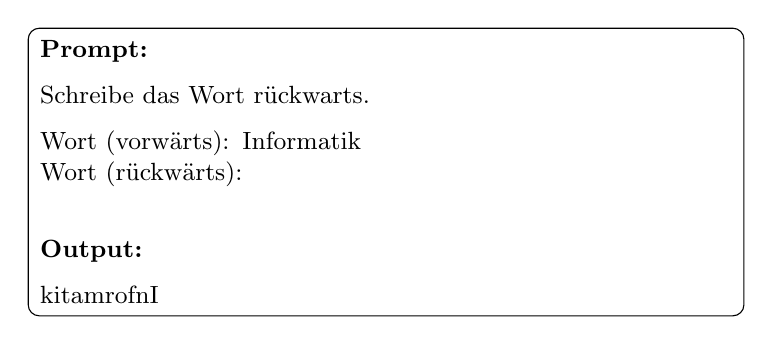
\begin{tikzpicture}
        \tikzset{node distance = 0.75cm and 1.5cm}
        % Main node with embedded tikzpicture
        \node (n1) at (0,0) [block] {
            \textbf{Prompt:}\\[0.2cm]

            Schreibe das Wort rückwarts.\\[0.2cm]
            Wort (vorwärts): Informatik\\
            Wort (rückwärts): \\[0.6cm]
            
            \textbf{Output:}\\[0.2cm]
            
            kitamrofnI};
    \end{tikzpicture}
    \caption{\textit{Zero-Shot Prompt} Beispiel}
    \label{fig:prompt-zero}
\end{figure}
\\Bei komplexeren Anforderungen kann es dazu kommen, dass ein \textit{Zero-Shot Prompt} nicht funktionert bzw. nicht zum erwarteten Ergebnis führt. In diesem Fall empfiehlt es sich, im \textit{Prompt} zusätzlichen Kontext in Form von Demonstrationen oder Beispielen hinzuzufügen. \cite{PromptEngineeringGuide}\\\\
\textbf{Few-Shot Prompt}\\[0.2cm]
\textit{Few-Shot Prompting} wird als Technik verwendet, um kontextbezogenes Lernen durch Demonstrationen und Beispiele, innerhalb des \textit{Prompts}, zu ermöglichen und dadurch das Modell zu einer besseren Leistung zu führen. Hierbei eröffnet sich die Möglichkeit, die Lösung der Aufgabe in eine gewünschte bzw. bestimmte Richtung zu steuern. Abbildung \ref{fig:prompt-one} zeigt ein Beispiel für einen \textit{Few-Shot Prompt}. \begin{figure}[ht]
    \vspace{.5cm}
    \centering
    \tikzstyle{block} = [rectangle, draw, text width=25em, inner sep=1ex, rounded corners, font=\small]
    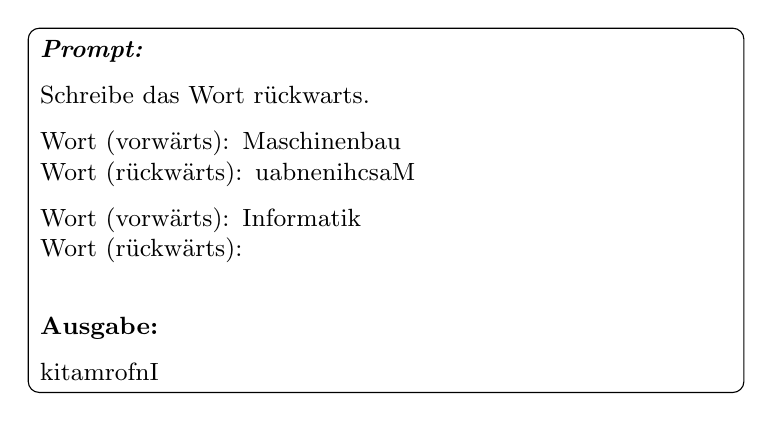
\begin{tikzpicture}
        \tikzset{node distance = 0.75cm and 1.5cm}
        % Main node with embedded tikzpicture
        \node (n1) at (0,0) [block] {
            \textbf{\textit{Prompt:}}\\[0.2cm]

            Schreibe das Wort rückwarts.\\[0.2cm]
            Wort (vorwärts): Maschinenbau\\
            Wort (rückwärts): uabnenihcsaM\\[0.2cm]
            Wort (vorwärts): Informatik\\
            Wort (rückwärts):\\[0.6cm]
            
            \textbf{Ausgabe:}\\[0.2cm]
            
            kitamrofnI};
    \end{tikzpicture}
    \caption{\textit{One-Shot Prompt} Beispiel}
    \label{fig:prompt-one}
\end{figure}
\\
Zusammenfassend lässt sich sagen, dass \textit{Prompt Engineering} Anweisungen nutzt, die ein \textit{fine tuning} der Leistung von vortrainierten LLM's basierend auf spezifischen \textit{Prompts} ermöglicht, und somit die Vielseitigkeit und Anwendung in unterschiedlichen Bereichen verbessert. \cite*{sahooSystematicSurveyPrompt2024}

\section{Unit Testing}
Ein Hauptproblem im Softwareentwicklungszyklus ist häufig die fehlende Zeit, um ein komplettes Projekt vor dem \textit{Release} manuell zu testen. \cite*{SoftwareQualityLab} Eine Lösungsvariante für diese Art von Problemstellungen bieten \textit{Unit-Tests}. 

\subsection{Grundlagen}
\textit{Unit-Tests} werden von Entwicklern geschrieben, um eine bestimmte Funktionalität in einem Ausschnitt des Codes zu testen. Somit wird es ermöglicht problematische Bereiche im Code offenzulegen und Fehler zu reduzieren. \cite*{tosunEffectivenessUnitTests2018} Die Tests werden in der gleichen Programmiersprache geschrieben wie der Produktionscode und bilden die Basis der \textit{Testing} Pyramide (Abb. \ref{fig:pyramid}). \begin{figure}[ht]
    \vspace{0.3cm}
    \centering
    \begin{tikzpicture}
        \coordinate (A) at (-3,0) {};
        \coordinate (B) at (3,0) {};
        \coordinate (C) at (0,4.75) {};
        \draw[name path=AC] (A) -- (C);
        \draw[name path=BC] (B) -- (C);
        \foreach \y/\A in {0/\textbf{\textit{Unit}},1/\textit{Integration},2/\textit{End-to-End},3/\textit{Manual}} {
            \path[name path=horiz] (A|-0,\y) -- (B|-0,\y);
            \draw[name intersections={of=AC and horiz,by=P},
              name intersections={of=BC and horiz,by=Q}] (P) -- (Q)
            node[midway,above] {\A};
    }
    \end{tikzpicture}
    \caption{Testing Pyramide}
    \label{fig:pyramid}
\end{figure}Idealerweise werden sie häufig und automatisiert durchgeführt, um sicherzustellen, dass neue Änderungen die bisherig bestehende Funktionalität nicht zerstören. \cite*{TestingPyramidStrategic2024}\\
Der Prozess des \textit{Unit-Testing} besteht aus grundlegend 4 Phasen. Die Planung dient zur Überlegung und Analyse, um entscheiden zu können welche Codeeinheiten getestet werden müssen. Dabei ist es essenziell alle relevanten Funktionen der Einheiten abzudecken. \cite*{bakharevUnitTestingDefinition2023} Die zweite Phase dient zum Schreiben der Testfälle, in der ein Skript angefertigt und Code für den \textit{Unit-Test} geschrieben wird. \cite*{bakharevUnitTestingDefinition2023} Beim Ausführen der Tests, welches die dritte Phase widerspiegelt, wird erkennbar, wie sich der Programmcode bei jedem Testfall verhält und eine Analyse ermöglicht (Phase 4), in der Fehler und Probleme im Code erkannt und behoben werden können.\cite*{bakharevUnitTestingDefinition2023}\\\\
Der \textit{Unit-Test} selbst, basiert meist auf einem 3A-\textit{Pattern}:
\begin{itemize}
    \setlength{\parskip}{0.5pt}
    \item \textit{Arrange} (engl. arrangieren)
    \item \textit{Act} (engl. agieren)
    \item \textit{Assert} (engl. behaupten)
\end{itemize}
\textit{Arrange} initialisiert die benötigen Objekte und setzt, wenn verlangt, \textit{mocks} (engl. Attrappen) um einen Platzhalter oder eine Attrappe für ein Objekt bereitzustellen.\\ Der \textit{Act}-Abschnitt ruft die zu testende Funktion mit den im vorherigen Schritt initialisierten Objekten auf und mithilfe des \textit{Assert}-Abschnitts wird überprüft, dass sich die Funktion wie erwartet verhält. \cite*{ikechiHowStructureUnit2021} [Quellcode \ref{lst:java-method-example} und \ref{lst:java-unit-example}]\\
\lstinputlisting[caption=\textit{Java}-Methode Beispiel,captionpos=b,label={lst:java-method-example},language=Java]{Assets/Code/Example-Func.java}\vspace{-.3cm}
Somit sind \textit{Unit-Tests} eine wichtige Maßnahme zur Qualitätssicherung und ermöglichen das frühzeitige Finden und Beheben von Fehlern.\\
\lstinputlisting[caption=\textit{Unit-Test} Beispiel,captionpos=b,label={lst:java-unit-example},language=Java]{Assets/Code/Example-Unit.java}\vspace{-.3cm}

\subsection{Java mit JUnit5}
\textit{JUnit} ist ein \textit{Unit-Testing-Framework}, welches zum Testen in \textit{Java} Anwendungen verwendet wird. Die aktuellste Version des \textit{Frameworks} ist \textit{JUnit5}, das eine moderne Grundlage für entwicklerseitige Tests bietet. \cite*{JUnit} \textit{JUnit5} unterstützt die automatisierte Durchführung von Tests und trägt somit zur Effizienzsteigerung aus Sicht des Entwicklungsprozesses bei. \cite*{venkatesanJunitFrameworkUnit} Es werden Werkzeuge und nützliche \textit{Features} zur Verfügung gestellt, um das Implementieren von Testfällen zuverlässiger und schneller zu gestalten. Einige der wichtigsten und am häufigsten verwendeten \textit{Features} sind dabei Annotationen, Testklassen und \textit{Assertions} (engl. Behauptungen). \cite*{venkatesanJunitFrameworkUnit}\\
Annotationen sind \textit{Tags}, welche zunächst dem \textit{Java}-Code hinzugefügt werden, um die Lesbarkeit und Struktur des Programmcodes zu verbessern. Ebenso definieren sie die Reihenfolge von Codeteilen innerhalb des Tests. Einige Beispielannotationen sind: \cite*{JUnitUserGuide}
\begin{itemize}
    \setlength{\parskip}{1pt}
    \item \textbf{\textit{@Test}} - zeigt, dass eine Methode eine Testmethode ist
    \item \textbf{\textit{@BeforeEach}} - legt fest, dass die Methode vor jedem \textit{@Test} ausgeführt wird
    \item \textbf{\textit{@AfterAll}} - legt fest, dass die Methode nach allen \textit{@Test} ausgeführt wird
\end{itemize}
Testklassen können mehrere Testmethoden beinhalten, was ein Ausführen von mehr als einer Testmethode vereinfacht und für strukturelle Vorteile wie die Lesbarkeit innerhalb des Projektes sorgt. Quellcode \ref{lst:java-class-example} zeigt ein Beispiel:\\
\lstinputlisting[caption=Testklasse Beispiel,captionpos=b,label={lst:java-class-example},language=Java]{Assets/Code/Example-Class.java}\vspace{-.3cm}
\textit{Assertions} finden in der Praxis häufig Anwendung und stellen weitere nützliche Methoden zum Schreiben von Testfällen dar. Einige der wichtigsten Methoden demonstriert Quellcode \ref{lst:assertions-example}.\\
\lstinputlisting[caption=Assertion-Methoden,captionpos=b,label={lst:assertions-example},language=Java]{Assets/Code/Assertions.java}\vspace{-.3cm}
Die einfachste Möglichkeit \textit{JUnit5} einzurichten, ist die Verwendung von \textit{Apache Maven}. Hierbei handelt es sich um ein weit verbreitetes \textit{Build-Automation-Tool} für \textit{Java}-Anwendungen. Zur Einrichtung reicht ein einfaches Hinzufügen der \textit{JUnit-Dependency} zum \textit{Project Object Model} (engl. kurz POM) in der \textit{pom.xml}. \cite*{baeldungGuideJUnitBaeldung2016}

\section{SonarQube}
In den vorherigen Kapiteln wurde deutlich, dass eine Testabdeckung des Projekts mit \textit{Unit-Tests} ein entscheidender Faktor für die Qualität des Programmcodes ist. Allerdings stellt sich die Frage, anhand welcher Kriterien sich die Qualität der Tests beurteilen lässt und wie sichergestellt werden kann, dass der Testcode die Anwendung tatsächlich umfassend abdeckt. Ein solches selbst verwaltendes und automatisches \textit{Code-Review-Tool} stellt \textit{SonarQube} bereit. Dabei lässt es sich in den bestehenden Arbeitsablauf integrieren und erkennt Probleme im Programmcode sowie im Testcode. \cite*{SonarQube10} Des Weiteren werden Metriken bereitgestellt, die eine Bewertung des eigenen Testcodes ermöglichen und dadurch eine Einschätzung der Abdeckung der Anwendung zulassen.\\\\
Eine erste entscheidende Metrik ist die \textit{Code Coverage} (engl. Codeabdeckung) der Tests. Anhand dieser \textit{Coverage} lässt sich die Frage beantworten, wie viel des Quellcodes durch \textit{Unit-Tests} abgedeckt wurde. Durch folgende Gleichung lässt sich eine Abdeckung in \% berechnen \cite*{MetricDefinition}:\\\\
$Coverage = \frac{(CT + CF + LC)}{2 \cdot B + EL}$
\begin{itemize}
    \setlength{\parskip}{1pt}
    \item CT - Bedingungen, die mindestens einmal als \textit{true} ausgewertet wurden
    \item CF - Bedingungen, die mindestens einmal als \textit{false} ausgewertet wurden
    \item LC - abgedeckte Quellcodezeilen
    \item B - Gesamtzahl an Bedingungen
    \item EL - Gesamtzahl an ausführbaren Quellcodezeilen
\end{itemize}
Im Allgemeinen wird eine Codeabdeckung durch \textit{Unit-Tests} von 60\% - 90\% angestrebt. \cite*{WhatReasonableCode}
Eine weitere Metrik, die zur \textit{Code Coverage} beiträgt, ist die \textit{Condtion Coverage} oder auch \textit{Branch Coverage} (engl. Bedingungs-/Zweigabdeckung). Hierbei wird zu jeder Quellcodezeile, die eine Verzweigung enthält, überprüft, ob der Ausdruck einmal für \textit{true} und einmal für \textit{false} ausgewertet wurde. Durch folgende Gleichung wird ein Ergebnis in \% ausgegeben \cite*{MetricDefinition}:\\\\
$Condition \,\, Coverage = \frac{(CT + CF)}{2 \cdot B}$
\begin{itemize}
    \setlength{\parskip}{1pt}
    \item CT - Bedingungen, die mindestens einmal als \textit{true} ausgewertet wurden
    \item CF - Bedingungen, die mindestens einmal als \textit{false} ausgewertet wurden
    \item B - Gesamtzahl an Bedingungen
\end{itemize}
Die \textit{Line Coverage} stellt ebenso ein Bestandteil der \textit{Code Coverage} dar und gibt an, wie viel \% der Quellcodezeilen durch die Tests ausgeführt werden \cite*{MetricDefinition}:\\\\
$Line \,\, Coverage = \frac{LC}{EL}$
\begin{itemize}
    \setlength{\parskip}{1pt}
    \item LC - abgedeckte Quellcodezeilen
    \item EL - Gesamtzahl an ausführbaren Quellcodezeilen
\end{itemize}
Wichtig ist, die Erfolgsquote der Tests auszuwerten. Dazu wird die Gesamtzahl der \textit{Unit-Tests} benötigt, um eine Quote angeben zu können. Man unterscheidet für die Berechnung zwischen \textit{Errors} und \textit{Failures}. Bei einem \textit{Unit-Test} Error handelt es sich um einen unerwarteten Fehler wie bspw. einem \textit{FileNotFound} Error wohingegen es sich bei einem \textit{Unit-Test Failure} um ein Fehlschlagen des Testfalls (bspw. bei einer falschen \textit{Assertion}) handelt. Die Quote selber, lässt sich wie folgt berechnen \cite*{MetricDefinition}:\\\\
$Success = \frac{(Tests - (Errors + Failures))}{Tests \cdot 100}$\\\\
Durch die oben genannten Metriken, lässt sich die Qualität der \textit{Unit-Tests} aus verschiedenen Blickwinkeln evaluieren.\\
Eine ausführliche Analyse benötigt eine Auswertung an sowohl simplen bis hin zu komplexen Projekten. \textit{SonarQube} stellt mit der \textit{Complexity} oder auch \textit{Cyclomatic Complexity} (engl. zyklomatische Komplexität) eine Metrik bereit, welche für eine spezifische Sprache die Komplexität berechnet. Diese wird durch die Anzahl an \textit{function splits} (engl. Funktionsaufteilungen) definiert. Für die Programmiersprache Java erhöht sich die Komplexität somit bei jedem \colorbox{gray!20}{if}, \colorbox{gray!20}{for}, \colorbox{gray!20}{while}, \colorbox{gray!20}{case}, \colorbox{gray!20}{\&\&}, \colorbox{gray!20}{||}, \colorbox{gray!20}{?} und \colorbox{gray!20}{->}. \cite*{MetricDefinition}
